\section{Experiment and Analysis}
\label{sec:experimentdesign}
To evaluate the spectrum utility from in-field measurements, we perform experiments 
with an off-the-shelf wireless platform and mobile spectrum analyzer.
%We collect measurements in typical populated areas and sparse areas of DFW metropolitan carrying these platforms. 
According to the measured data, we apply our MAPE framework to analyze the role
of white space and WiFi bands in total access points required for a given deployment area.

\subsection{Experiment Design}
% Platform
%To ensure the results are applicable, 
We employ a Linux-based 802.11 testbed, which includes a Gateworks 2358 board with 
Ubiquiti XR radios (XR9 at 900 MHz, XR2 at 2.4 GHz, XR5 at 5.2 GHz) and a DoodleLabs DL475 
radio at 450 MHz.  We develop shell scripts with tcpdump for this testbed working as a sniffer 
and recording all 802.11 packets. However, since the Gateworks platform only updates its
estimate of received signal strength upon the reception of a new packet, we employ a
a spectrum analyzer to form a notion of inter-network interference with finer granularity.
We have Rohde \& Schwarz FSH8 portable spectrum works from 100 KHz to 8 GHz. The portable spectrum
analyzer is controlled by a Python script on a laptop measure the received signal strength 
in a short term. 
%We perform experiments in downtown Dallas, SMU campus, and neighborhood. The results show
%no 802.11 packets detected in white space bands(450 MHz, 900 MHz) there. 
%And in DFW area, as far as we know, we are the only group holds FCC license of white space bands. 
%Our experiments verify that these bands have not been used for commercial wireless data communication.
%Moreover, we observed that Gateworks platform only update its received signal strength when received
%a new packet.
%It is not good for inter-network interference measurement. To cover the gap,
%we employ a spectrum analyzer, multiband antenna, mobile antenna and a laptop developing
%a spectrum sensing system.

% Data normalize 
As far as we know, there is no mobile multiband antenna in the market. We use a 700 MHz
mobile antenna to perform the in-field experiments. 
Then, we uniform the mobile antenna 
measurements across bands by comparing with the indoor measurements from the multiband antenna
with our controlled signal source. First we use USRP(Universal Software Radio Peripheral) 
N210 to generate signals in 450 MHz, 800MHz, and 2.4 GHz~\cite{usrp}. We feed the USRP 
signals directly to a spectrum analyzer and adjust the configuration of USRP to make
the received signal strength the same as the 5.2 GHz signal from Gatework 2358 with 
a XR5 radio. Then we connect the signal source to the multiband antenna, and measure the 
received signal in a fixed distance with the 700 MHz antenna and antennas for different bands
to get the antenna loss of all the bands. Then we normalize the received signal strength 
collected through 700 MHz mobile antenna.

  \begin{figure}
  %\vspace{-0.0in}
  \centering
  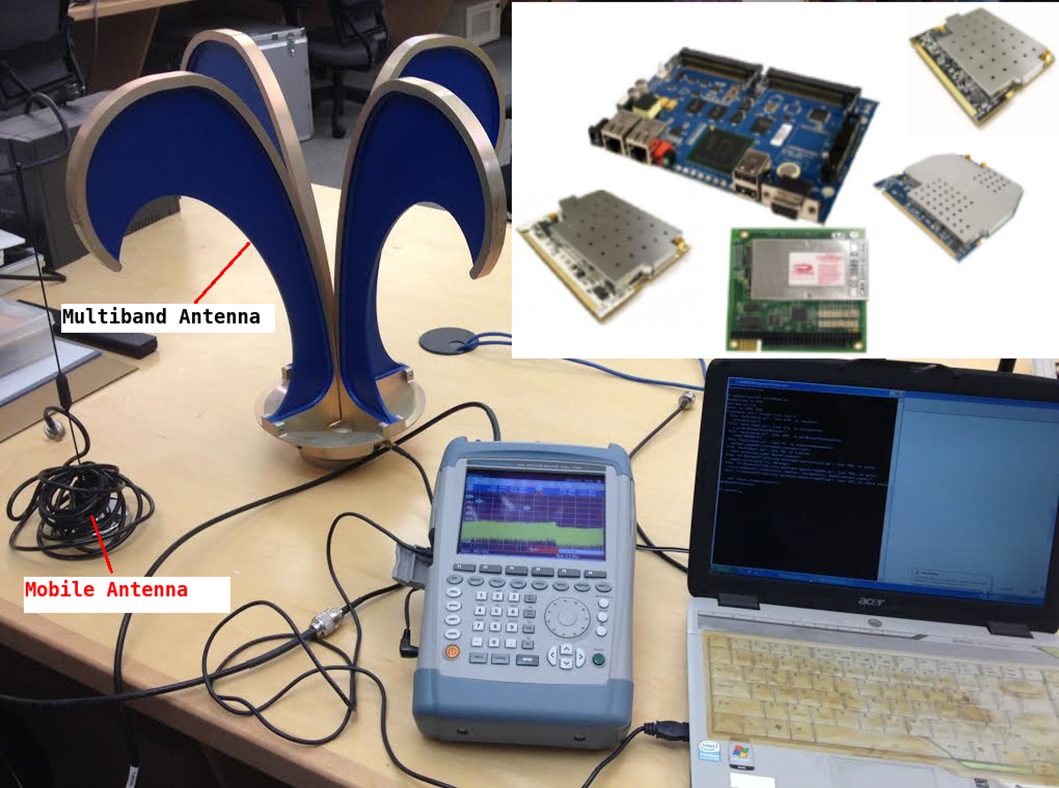
\includegraphics[width=74mm]{figures/equipment}
  \vspace{-0.1in}
  \caption{Multiband Measurement Platform}
  \label{fig:equipment}
  \vspace{-0.15in}
  \end{figure}
  
% Duplicate measurement in WiFi
Our experiment platforms are shown in Figure~\ref{fig:equipment}.
We have 32 samples each second for each band from the spectrum analyzer with time stamps.
Gateworks sniffer platform records all the packets received in WiFi bands with time stamps. 
The duplicated samples in WiFi bands from spectrum analyzer and Gateworks are deleted 
according to the time stamp. Then we use the data for activity level calculation in WiFi bands. 
The activity level of white space bands is calculated based on the spectrum analyzer measurements.  

% Location and Process 
%We apply drive test carrying our platform from Dallas to Weatherford as shown in~\ref{sec:problemformulation}.
We choose experiments locations according to the population distribution in DFW metropolitan. 
The experiments are performed in Dallas, Weatherford and Millsap marked with stars in 
Figure~\ref{fig:drivemap}.
We have collected measurements at multiple locations, including the neighborhood, campus and 
urban area in Dallas.
In Weatherford and Millsap, we monitor wireless activities in three locations for 45 minutes
on a normal weekday. 
Downtown, neighborhood and rural area are chosen from Weatherford and Millsap. 
Then we post-process the data to calculate the activity level of each band in each location.


\subsection{Results and Analysis} 
\label{subsec:result}
In this subsection, we discuss our measurements results and perform our WAPE framework 
to analyze the influence of white space channels across areas with different population densities.

Figure~\ref{fig:drivemap} depicts a map of the available white space channels with
markers where we performed measurements in North Texas. To be representative of a broad range of 
community types, we consider populations of approximately 25 times one another according to the
2010 U.S. Census, Millsap (500), Weatherford (25k), and Dallas (1.25 M). 

As an initial experiment, 
we perform a drive test from Dallas to Weatherford with cruise control set to 60 MPH while on
the highway.  
Part of the result of in-field spectrum measurement is shown in Figure~\ref{fig:drivetest}.
The measured RSSI of 450 MHz is strong in downtown Dallas, downtown Fort Worth;
but has less signal activity in the urban and rural area between these cities.
The low activity detected in WiFi bands is due to the distance from highway is larger
than the propagation range of an indoor wireless router whose transmitting power is limited.
The map itself shows the available white space channels in DFW area, more green means
more channels. Our in-field measurement matches the FCC restriction showing that less channels means
more spectrum utility and tell the spectrum utility levels varying across population 
distribution. We use the measurements collected at more fixed locations as marked on the map for
the activity level calculation. 

\begin{figure}
%\vspace{-0.0in}
\centering
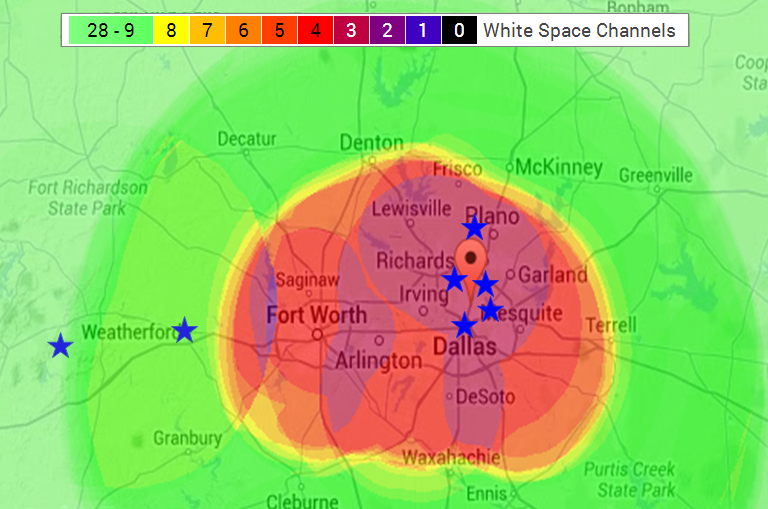
\includegraphics[width=74mm]{figures/drivemap}
\vspace{-0.1in}
\caption{DFW Metropolitan Measurement Location}                                                                 
\label{fig:drivemap}
\vspace{-0.1in}
\end{figure}
   
\begin{figure}
%\vspace{-0.0in}
\centering
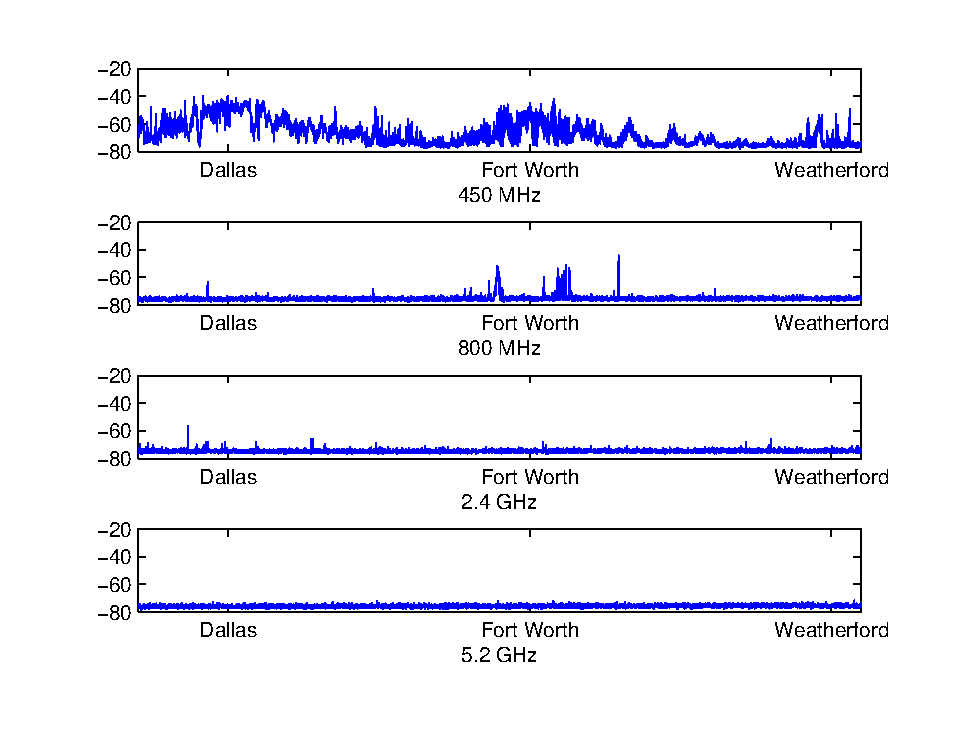
\includegraphics[width=94mm]{figures/drivetest}
\vspace{-0.1in}
\caption{Spectrum Activity In DFW}                                                                 
\label{fig:drivetest}
\vspace{-0.1in}
\end{figure}

The activity level calculated with our measurements are shown in Table~\ref{tab:activitymeasurement}.
Dallas as the central city of North Texas, has the highest activitie level in most of the measured bands,
especially in 450 MHz. The measurements of Dallas urban are taken from SMU campus, 2 neighborhoods
and city Plano. Our meaurements indicates that 2.4 GHz has a higher activity level in urban area than 
downtown area. Most schools and their neighborhoods are covered by WiFi today,
which explains the high activity level in 2.4 GHz and 5.2 GHz.
In Weatherford, all the bands have lower activity levels than in Dallas. And due to the location for 
measurement collection, the rural area on the west of Weatherford could receive more 
interference from Fort Worth.
Millsap is a typical sparse city with 500 residents total in north Texas. The activity levels across 
all the bands are lower than in Dallas and Weatherford. In 450 MHz band, the activity level decreases 
much faster than in other bands in Dallas and Weatherford. 



%% Fix location example claiming the activity is kind of stable
%Figure~\ref{fig:labact} depicts an example spectrum utility in activity level
%defined in~\ref{subsec:problem} in our urban lab with the platform introduced 
%in~\ref{sec:experimentdesign}. 
%The activity level from data collected in the same location shows 
%the difference in time domain. On average, the existing signals occupy 25.83 
%percentage of time in 450 MHz, 26.49 percentage of time in 800 MHz, 
%34.95 percentage of time in 2.4 GHz and 35.46 percentage of time in 5.2 GHz. 
%Our experiments show that in a fixed location, the spectrum utility is around
%a certain number in time domain. This character provides a method to tell
%the spectrum utility through measurements. These Inter-network interference 
%of existing signals have to be counted in wireless network deployment. 
%
%   
%In the measurements, there is around $10\%$ difference from white space 
%band to WiFi bands in our urban lab. This spectrum utility gap and multiband
%propagation variation in band selection of wireless network 
%deployment is what we have to notice. 
%




\begin{table*}
\centering % centering table 
\begin{tabular}{|l|c|c|c|c|c|c|c|c|c|c|c|} % creating 12 columns 
\hline %\hline % inserting double-line 
Bands     & \multicolumn{3}{c|}{Dallas} & \multicolumn{3}{c|}{Weatherford} & \multicolumn{3}{c|}{Millsap} \\% [0.5ex]
\hline % inserts single-line 
% Entering 1st row 
Area Type & Downtown & Urban & Sparse Area & Downtown &  Urban   & Sparse Area & Downtown & Urban & Sparse Area \\ % [0.5ex]
\hline % inserts single-line 
450 MHz &24.37	&25.83  &23.77	&6.05 &12.50  &14.03 & 7.00 & 0.07 & 0.02 \\      
\hline % inserts single-line                                                                                                       
800 MHz &4.40 	&16.49  &4.77	&5.22&5.07 &4.43  & 3.87 & 4.20 & 3.60 \\      
\hline % inserts single-line                                                                                                      
2.4 GHz &15.87 	&34.95  &2.60	&2.03&2.03 &2.77  & 2.07 & 1.60 & 0.80 \\      
\hline % inserts single-line                                                                                                     
5.2 GHz &19.70	&35.46  &1.53	&1.93&1.93 &1.33  & 1.27 & 2.07 & 2.10 \\      
\hline % inserts single-line 
\end{tabular}    
\label{tab:activitymeasurement}    
\caption{Activity Level in Multiple Locations} % title name of the table 
\vspace{-0.1in}
\end{table*}    

We put these measurement based activity level into our framework presented in 
Algorithm~\ref{algorithm:mape}. We use Millsap
sparse area, Millsap downtown, Weatherford urban, Dallas urban, and Dallas downtown measurement as input activity level
map to the population density.
We input these information to our framework and calculate the number of access point for covering 
a $13 km \times 13 km$ area varying population density. The output is shown in Figure~\ref{fig:redensity}. 

   \begin{figure}
   %\vspace{-0.0in}
   \centering
   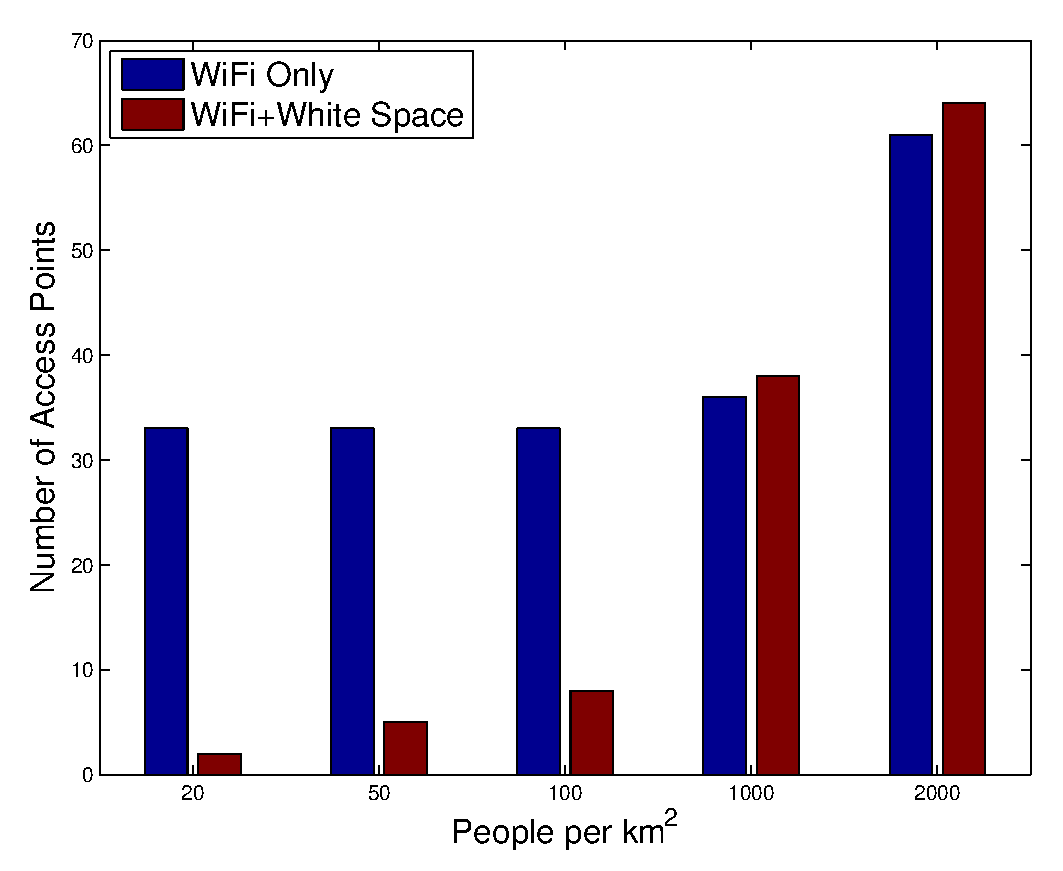
\includegraphics[width=74mm]{figures/redensity}
   \vspace{-0.1in}
   \caption{Number of Access Points need for 13x13 $km^2$ Area}
   \label{fig:redensity}
   \vspace{-0.1in}
   \end{figure}

% Experiment Results & expect results
In the calculation, we set the demand request as $2\ Mbps$ per person, the population
density as $20,50,100,1000,2000$ per square kilometers. We assume $30\%$ residents will use this
service, the maximum transmit power $30 dBm$, path loss exponent $3.5$~\cite{meikle2012global}. 
For WiFi only, we use 6 channels in 2.4 GHz, and 3 channels in 5.2 GHz. 
Our experiment platforms are shown in Figure~\ref{fig:equipment}.
We adopt 802.11n maximum data rate 600 Mbps. For WiFi+ White Space
scenario, we use 3 channels in 450 MHz, 2.4 GHz and 5.2 GHz each. Then all the scenarios have the 
same channels in total. As shown in Figure~\ref{fig:redensity},
with the same number of channels, WiFi+White Space gains $1650\%$ comparing to WiFi only in 20 people 
per square kilometer scenario, and $660\%$ in 50 people per square kilometer and $412.5\%$ in 100 people
per square kilometer. But as the population density increase, due to the capacity constraint servicing
people in this area, low frequency white space band lose their advantage of larger communication range. 
And at the same time, the activities of other signal source, such as TV station in downtown area reduce
the capacity of white space band, then WiFi+White Space bands perform worse than WiFi only bands combination.
If we count the intra-network interference which is out of our scope, the situation could be even worse.
Moreover, FCC has stricter policy of white spaces in downtown and urban area. Fewer channels
are available in these area which make WiFi bands a better option for population dense areas.

To find the bands combination influence on network deployment, we calculate the number of access
points in the area. We select 500 people per square kilometer with Weatherford 
downtown spectrum utility, and 1500 people per square kilometer with Dallas urban spectrum utility
running numerical analysis. We assume the total number of channels is 12. We use the same setup 
as the previous experiment. The results are shown in~\ref{tab:500comb}.
 
 
 \begin{table}[h]
 \centering
 \begin{tabular}{|c|c|c|c|}
 \hline
 \multirow{2}{*}{No. of Bands} & \multirow{2}{*}{Bands Combination} & \multicolumn{2}{c|}{No. of AP} \\
 \cline{3-4}
  &  & 500 & 1500 \\
 & (Hz) & population &  population \\
 \hline
 \multirow{4}{*}{1}    & 450 M  & 12  & 35 \\
 \cline{2-4}
                              & 800 M & 10  &  30 \\
 \cline{2-4}
			      & 2.4 GHz & 33  &  37 \\
 \cline{2-4}
                              & 5.2 G & 193 &  193 \\ 
 \hline
 \multirow{6}{*}{2}   & 450 M,800 M & 11  & 32\\
 \cline{2-4}
                              & 450 M,2.4 G & 23  & 36\\
 \cline{2-4}
			      & 450 M,5.2 G & 23  & 69\\
 \cline{2-4}
			      & 800 M,2.4 G & 20  & 33\\ 
 \cline{2-4}
			      & 800 M,5.2 G & 20  & 59\\ 
 \cline{2-4}
			      & 2.4 G,5.2 G & 33  & 73\\ 
 \hline
 \multirow{4}{*}{3} & 450 M,800 M,2.4 G & 16  & 33\\
 \cline{2-4}
                              & 450 M,800 M,5.2 G & 16  & 48\\
 \cline{2-4}
			      & 450 M,2.4 G,5.2 G & 33  & 53\\
 \cline{2-4}
			      & 800 M,2.4 G,5.2 G & 30 &  49\\ 
 \hline
 4  & 450,800 M,2.4,5.2 G & 21  & 44 \\
 \hline
 \end{tabular}
 \caption{Channel Combinations for $500$ and $1500$ Population Density Scenarios}
 \label{tab:500comb}
 \end{table}


In the table, we compare the number of access points with 12 channels through all 
the possible combinations of bands. 
% Single band compare
When all the channels are in the same band. as frequency goes up, more access 
points are need to serve the area due to the limited propagation range. 
450 MHz does not outperform 800 MHz in single band at both 500 and 1500 population
density cases because 450 MHz channels have larger measured activity level in experiment setup. 
White space band channels outperform WiFi bands up to 1830\% in single band case
at 500 population density. But in 1,500 population density, the gain decrease to 543.33\%.
% Two bands 
We distribute equal number of channels to 2 bands combinations and run the experiments in 
two population and spectrum utility scenarios. The numerical results shows white space bands 
combination(450 MHz,800 MHz) performs better than WiFi only(2.4 GHz, 5.2 GHz) by 200\% in 
500 population density and 128.12\% in 1,500 population density. 
White space only(450 MHz, 800 MHz) has almost the same performance as white space + WiFi 
scenario(450 MHz, 2.4 GHz; 800 MHz, 2.4 GHz) in 1,500 population density. But in 500 population
density, white space only is much better than any other 2 bands combinations.
% Three bands
White space channels brings up to 87.5\% gain in 3 bands combination scenario in 500 population
density and up to 33.3\% gain in 1,500 population density. And with 4 bands, the number of 
access points does not outperform using channels in white space bands.

From figure~\ref{fig:redensity} and Table~\ref{tab:500comb}, we could find as the population
density increase, the gain of white spaces decrease. Centralizing channels in white space
bands could get more benefit comparing with distribute them into multiband bands.
And also, as population and spectrum utility increase, at some point, the performance of
white space only could be the same as white space+WiFi combination. Then we may pay
less money to get less number of white space channels for wireless net work deployment.

